\documentclass[a4paper,10pt]{article}

\usepackage[brazilian]{babel}
\usepackage[utf8]{inputenc}
\usepackage{titlesec}
\usepackage{graphicx}
\usepackage{mathtools}
\usepackage{amsthm}
\usepackage[top=1.0in,bottom=1.0in]{geometry}
\usepackage{hyperref}
\usepackage[singlelinecheck=false]{caption}
\usepackage[backend=biber,url=true,doi=true,eprint=false]{biblatex}
\usepackage{enumitem}
\usepackage[x11names, rgb]{xcolor}
\usepackage{tikz}
\usepackage{abstract}
\usepackage{indentfirst}
\usepackage[justification=centering]{caption}

\usetikzlibrary{snakes,arrows,shapes}

\addbibresource{references.bib}

\newcommand\blfootnote[1]{%
  \begingroup
  \renewcommand\thefootnote{}\footnote{#1}%
  \addtocounter{footnote}{-1}%
  \endgroup
}

\DeclareMathOperator*{\argmin}{arg\,min}
\DeclareMathOperator*{\argmax}{arg\,max}

\newcommand\defeq{\mathrel{\overset{\makebox[0pt]{\mbox{\normalfont\tiny\sffamily def}}}{=}}}

\renewcommand{\abstractnamefont}{\normalfont\Large\bfseries}

\titleformat{\section}
  {\normalfont\scshape\bfseries}{\thesection}{1em}{}
\titleformat{\subsection}
  {\normalfont\scshape\bfseries}{\thesubsection}{1em}{}
\titleformat{\paragraph}
  {\normalfont}{\theparagraph}{1em}{}
\titleformat{\subparagraph}
  {\normalfont}{\thesubparagraph}{1em}{}

\captionsetup[table]{labelsep=space}

\theoremstyle{plain}

\newtheorem*{thm-def}{Definição}
\newtheorem*{thm-thm}{Teorema}

\setlength{\parskip}{1em}

\begin{document}

\begin{titlepage}
  \begin{center}
    \LARGE
    \textbf{Jogando Atari e (S)NES com Aprendizado de Máquina e Redes Neurais}

    \vspace{1.7cm}
    \Large
    Um estudo superficial sobre automatização de jogos com aprendizado baseado em reforço e
    redes neurais artificiais

    \vspace{1.7cm}
    \Large
    Renato Lui Geh

    \vfill
    \Large
    Universidade de São Paulo

    Instituto de Matemática e Estatística

    Monografia para MAC0412
    \vspace{1.5cm}
  \end{center}
\end{titlepage}

\newpage
\null\vspace{\fill}
\begin{abstract}
  \large
  A proposta deste trabalho é apresentar os conceitos de aprendizado baseado em reforço com o uso
  de processos de decisão markovianos, redes neurais artificiais, como aplicar aprendizado em redes
  neurais, as especificações de \textit{hardware} tanto do Atari 2600 quanto do NES e finalmente
  uma proposta de como aplicar aprendizado em um agente jogador automático.

  Este trabalho foi baseado no artigo da Google DeepMind \textit{Human-level control through deep
  reinforcement learning}\cite{mnih-et-al}, onde Mnih \textit{et al} explicam um novo algoritmo de
  aprendizado de Q-networks profundas que teve melhor performance em experimentos realizados no
  Atari 2600 do que outros algoritmos. O artigo \textit{The First Level of Super Mario Bros. is
  Easy with Lexicographic Ordering and Time Travel... \small{after that it gets a little tricky}}
  \cite{dr-murphy}, que explica como extrair uma função objetivo a partir da memória usada em
  plataformas NES, também teve grande influência nesta monografia.

  Nesta monografia serão primeiro apresentados os conceitos de aprendizado de máquina, processos
  de decisão markovianos, aprendizado baseado em reforço e redes neurais artificiais nesta ordem.
  Em seguida serão apresentadas as diferenças entre o método de automatização usado em Mnih
  \textit{et al} e o apresentado em \textit{Murphy}.
\end{abstract}
\vspace{\fill}
\newpage
\large
\tableofcontents
\normalsize
\newpage
\section{Introdução}

A monografia é dividida em 5 tópicos: introdução, noções fundamentais de probabilidade, processos
de decisão markovianos, aprendizado baseado em reforço, redes neurais artificiais, hardware e
finalmente automatização de um agente jogador.

Quando dizemos um agente jogador automático, queremos dizer um agente que performe de forma
racional e ótima no contexto do jogo. Um agente jogador automático ideal não é restringido por
regras específicas de um dado jogo, mas performa de forma ótima em todos os jogos. Por exemplo,
se o agente está jogando \textit{Breakout} de forma ótima, então o mesmo agente deve se comportar
de forma ótima em um outro jogo (por exemplo \textit{Montezuma's Revenge}) sem nenhuma
modificação no código.

\begin{figure}[h]
  \centering{
    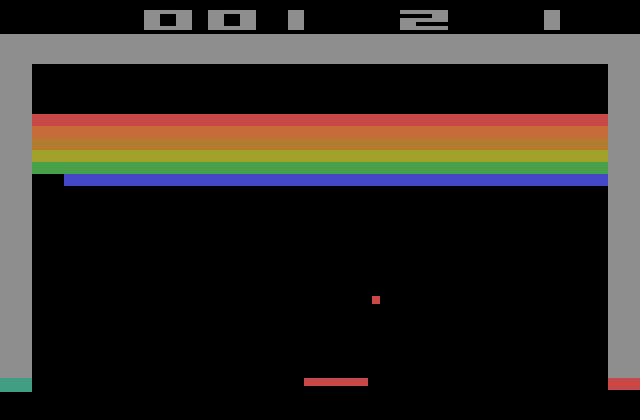
\includegraphics[scale=0.3]{imgs/breakout.png}
    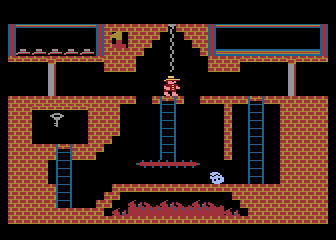
\includegraphics[scale=0.525]{imgs/montezuma.png}
    \caption{\textit{Breakout} (à esquerda) e \textit{Montezuma's Revenge} (à direita) no Atari
    2600. \textit{Fonte:} \url{http://en.wikipedia.org/} e \url{http://www.atariprotos.comi/}}
  }
\end{figure}

Infelizmente, tal agente não existe ainda. De fato, Mnih \textit{et al}\cite{mnih-et-al} mostram,
por meio de experimentos, que o agente teve um desempenho impressionante em \textit{Breakout},
mas foi muito mal em \textit{Montezuma's Revenge}. Isso é dado pela variedade de controles,
objetivos e condições de recompensa que cada jogo possue. Um agente ideal conseguiria aprender
todos os elementos de um jogo tal como um jogador humano dados todos estímulos visuais do próprio
jogo. No entanto, isso implica no reconhecimento de elementos específicos da tela como o domínio
de uma função que mapeia estímulos visuais a uma recompensa (seja imediata ou a longo prazo).

Uma outra alternativa seria o uso dos bits ``crus'' do próprio jogo para determinar que um objeto
seja mapeado na função objetivo (recompensa). Esta abordagem, no entanto, não indica que o agente
está sendo ``inteligente'' \footnote{A questão de um agente ser inteligente ou não é uma questão
mais filosófica e que requer um estudo muito mais aprofundado do que o que é exposto nesta
monografia}, mas que está apenas seguindo, de forma gulosa, a melhor recompensa direta a partir
de uma função já existente.

A diferença da abordagem visual e da abordagem ``crua'' pode ser comparada a um agente aprender
vendo vários vídeos de pessoas jogando um certo jogo ou aprender lendo um manual que aponta
exatamente quais ações o jogador deve tomar para que seu desempenho seja ótimo. Enquanto que os
dois métodos consistem na maximização das ações para gerar o melhor resultado, a abordagem visual
é um método muito mais geral e semelhante a como humanos se comportam. Além disso, a abordagem
crua depende da especificação do hardware e do jogo. Nesta monografia abordaremos principalmente
pelo lado visual, já que queremos um agente que seja independente da implementação usada.

\subsection*{Noções de Probabilidade}

O uso de probabilidades na área de Inteligência Artificial não foi imediata. A princípio, o método
preferível de se representar conhecimento era por meio de lógicas. Para representarmos algo que
existisse consideraríamos algum evento como verdadeiro. Uma relação de causa-efeito é dada por uma
implicação. Por exemplo, se desejássemos representar um mundo onde todo ser que come grama é uma
cabra, e que todo ser que come carne é urso, então diríamos que nossa base de conhecimento é
composta por:

\begin{align*}
  &Cabra, \quad Urso \\
  &Grama, \quad Carne \\
  &Come(X, Y) \\
  &\forall X, Come(X, Grama) \to Cabra \\
  &\forall X, Come(X, Carne) \to Urso
\end{align*}

No entanto, é fácil notar que quanto mais seres incluírmos no nosso mundo, mais regras precisamos
criar. Além disso no mundo anterior consideramos que um ser come grama se e somente se o ser é uma
cabra, e um ser come carne se e somente se o ser é um urso. Porém, digamos que existe um ser
chamado humano que come tanto grama quanto carne. Precisamos criar regras que diferencie um urso de
um humano e um humano de uma cabra. As lógicas mais tradicionais não conseguem lidar com elementos
que se justapõem sem diferenciarmos explicitamente com regras. De fato, uma das maiores
desvantagens da lógica é a enumeração exaustiva de todas as regras.

Podemos resolver este problema por meio de probabilidades. Considere o mundo anterior e digamos que
existe uma população de 60 cabras, 30 ursos e 10 humanos neste mundo. Então podemos construir a
seguinte tabela de probabilidades condicionais:

\begin{table}[h]
  \begin{center}
    \begin{tabular}{l | c  c}
      Animal & $P(Animal=x | Come=grama)$ & $(Animal=x | Come=carne)$ \\
      \hline
      Cabra & 0.857 & 0.00 \\
      Humano & 0.143 & 0.250 \\
      Urso & 0.00 & 0.750 \\
    \end{tabular}
  \end{center}
\end{table}

A primeira coluna categoriza um $Animal$ como uma das três possíveis opções: Cabra, Humano e Urso.
Cada $i$-ésima linha mostra a probabilidade condicional de $Animal$ ser $x$ dado que o que ele come
é grama ou carne. Note que toda coluna de probabilidades deve somar 1. Isto ocorre por que
temos conjuntos exaustivos que cobrem o nosso mundo inteiro. Para toda comida, o animal relativo
a ele deve estar contido em alguma população de animal.

Chamamos as probabilidades condicionais da forma $P(X=\{x_1,...,x_n\} | E=\{e_1,...,e_n\})$ de
probabilidades posteriores, onde $X$ é o conjunto de variáveis e $E$ é o conjunto de evidências
(variáveis observáveis do nosso mundo). As probabilidades da forma $P(X)$ são chamadas de
probabilidades \textit{a priori}.

\section{Aprendizado de Máquina}

Aprendizado de máquina pode ser visto como um jeito de aproximar uma função dados valores da função
somados a um erro. Ou seja, queremos uma função que minimize o erro dos valores dados com os
valores obtidos pela função. Por exemplo, na função dada pela Figura 2, queremos uma função que
consiga achar uma aproximação dos mesmos valores obtidos nos pontos azuis. Chamamos os pontos
azuis -- ou seja, os dados observados -- de conjunto de treino, já que iremos usar estes pontos
para treinar uma função para que ela consiga achar uma predição de menor erro possível para outros
pontos.

Em outras palavras, queremos achar uma função $f$ tal que:

\begin{equation*}
  f(x) = \argmin_{a, b} \sum_i (y_i - ax_i + b)^2
\end{equation*}

\newpage

\begin{figure}[h]
  \centering{
    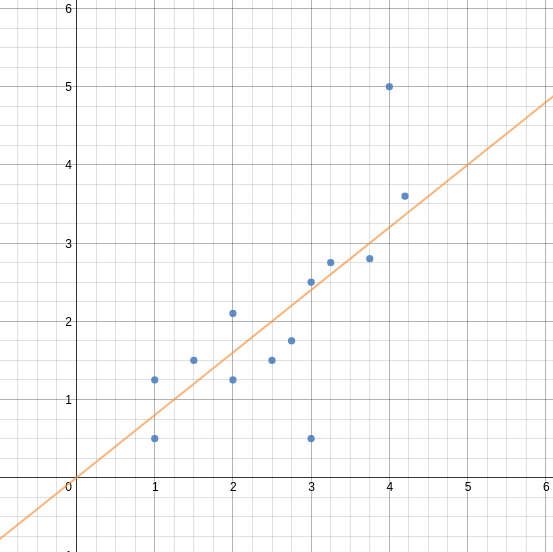
\includegraphics[scale=0.35]{imgs/learn_graph1.png}
    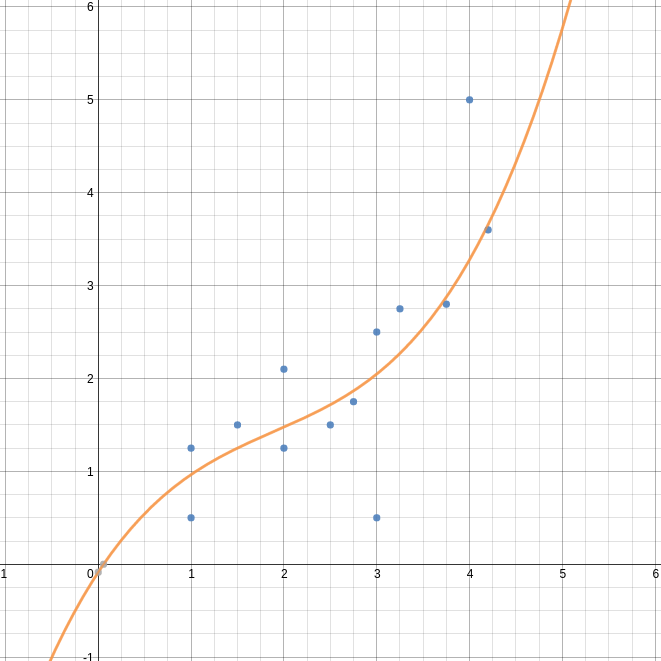
\includegraphics[scale=0.2915]{imgs/learn_graph2.png}
    \caption{Dados os valores de treino dado pelos pontos azuis no grafo, queremos uma função que
    minimize o erro $\sum_i (y_i - f(x_i))^2$ (dada pela função laranja).}
  }
\end{figure}


A partir de um conjunto de treino, podemos formular diferentes funções. Por exemplo, na Figura 2
podemos usar tanto a função à esquerda quanto à direita. Na função linear há um erro grande
entre $(5, 4)$ e $f(5)$, enquanto que na função à direita o erro é menor em $x=5$, mas o erro
é maior em outros pontos. A complexidade de uma função não depende somente do conjunto de treino,
mas também do conjunto de testes, ou seja, do conjunto que vamos tentar aproximar depois de termos
treinado a função. Um conjunto de testes que tenha valores excepcionais ou completamente diferentes
do conjunto de treino terá, obviamente, valores com alto erro. Precisamos, portanto, escolher um
conjunto de treino que, preferencialmente, cubra uma grande parte dos casos.

Se tentarmos especializar demais a função no conjunto de treino, o aprendizado sofrerá \textit{
overfitting}, ou seja, a função estará viesada demais, e provavelmente terá uma performance ruim
quando exposta a valores novos. O caso contrário, \textit{underfitting}, ocorre quando não temos
um conjunto de treino que cobre uma parte razoável dos possíveis valores.

\section{Processos de Decisão Markovianos}

\newpage
\printbibliography

\end{document}
